\section{Experimental Evaluation}
\label{sec:exp}

{\bf Experimental environment.} All experiments in this section were
conducted on a 16-slave in-house Open Stack cloud, using Linux Ubuntu
14.04 and Spark v1.6.  Each node has 4 cores and 16 GB of RAM.  Spark
Standalone cluster manager and Hadoop 2.6 were used.

Because Spark is a lazy evaluation system, a materialize operation was
appended to the end of each query, which consisted of the count of
nodes or edges.  Each experiment was conducted 3 times with a cold
start, we report the average running time, which is representative
because we took great care to control variability.  Standard deviation
for each measure is at or below 5\% of the mean except in cases of
very small running times.

\begin{table}
\caption{Experimental datasets.}
\small
\begin{tabular}{l | c | c | c | c }
\hline
\multicolumn{1}{l|}{\bfseries Dataset} & \multicolumn{1}{c|}{\bfseries |V|} & \multicolumn{1}{c|}{\bfseries |E|} & \multicolumn{1}{c|}{\bfseries Time Span} & \multicolumn{1}{c}{\bfseries Evol. Rate} \\ \hline
wikitalk-en & 2.9M & 10.7M & 2002--2015 & 14.4 \\ \hline
nGrams & 29.3M & 2.5B & 1520--2008 & ? \\ \hline
DELIS & 128M & 40.5B & 2006--2007 & ? \\ \hline
twitter & 505.4M & 23B & 2006--2012 & ? \\ \hline
\end{tabular}
\label{tab:datasets}
\end{table}

{\bf Data.}  We evaluate performance of our framework on four real
open-source datasets: wikitalk, nGrams, DELIS, and Twitter
(Table~\ref{tab:datasets}).  wikitalk~\cite{wikitalk} contains over 10
million messaging events among 3 million wiki-en users from 2002
through 2015, aggregated at 1 month resolution.  nGrams~\cite{nGrams}
contains word co-occurrence information from 1520 through 2008, with
30 million word nodes and over 2.5 billion undirected co-occurrence
edges.  twitter~\cite{twitter} contains over 23 billion directed
follower relationships between 0.5 billion twitter users collected in
2012, sampled at 1-month resolution based on account creation
information from April of 2006.  DELIS contains monthly snapshots of a
portion of the Web graph focusing on the .uk domains from 05/2006
through 05/2007~\cite{BSVLTAG}.  The datasets differ not only in size,
but also in the number and type of attributes and the rate of
evolution.  The change rate was calculated as the average graph edit
similarity~\cite{Ren2011}.  \eat{the evolutionary properties:
  co-authorship network nodes and edges have limited lifespan, while
  the nGrams network grows over time, with nodes and edges persisting
  for long duration.  All figures in the body of this section are on
  the larger nGrams dataset.  Refer to the Appendix for the DBLP
  figures, which show similar trends as nGrams.}

Our file format is Apache Parquet archives, one for vertices and
another for edges, time-coalesced.  This is a direct physical
translation of the vertex-edge \tg logical data model where the
attributes are stored with the topology.  In cases where there is 0 or
1 attribute per node/edge, such as in our datasets, this is also the
most compact representation.  If the input data is in uncoalesced
snapshots, then it occupies space as a function of the graph evolution
rate.  The behavior of the four physical representations reported
below is dependent on the underlying data format on disk and should be
interpreted in that context.

\begin{figure*}
\centering
\begin{minipage}{2.2in}
\centering
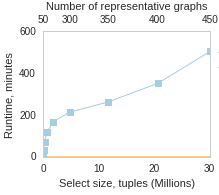
\includegraphics[width=2.2in]{figs/slice_ngrams_vertices_build11_trimmed.png}
\vspace{-0.1in}
\caption{Slice on nGrams dataset, return vertices.}
\label{fig:sliceverts}
\vspace{-0.1in}
\end{minipage}
\begin{minipage}{2.2in}
\centering
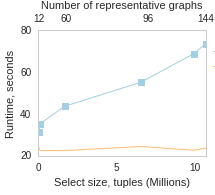
\includegraphics[width=2.2in]{figs/slice_wikitalk_edges_build11_trimmed.png}
\vspace{-0.1in}
\caption{Slice on wikitalk dataset, return edges.}
\label{fig:sliceedges}
\vspace{-0.1in}
\end{minipage}
\begin{minipage}{2.2in}
\centering
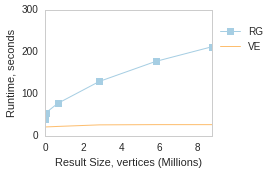
\includegraphics[width=2.6in]{figs/project_wikitalk_vertices_build12.png}
\vspace{-0.1in}
\caption{Project on wikitalk dataset vertices.}
\label{fig:project}
\vspace{-0.1in}
\end{minipage}
\end{figure*}

{\bf Slice.}  \insql{slice} performance was evaluated by varying the
slice time window and materializing vertices or edges.  Recollect that
in \ve \insql{slice} is a simple select on the vertex and edge
relations and is the fastest access method when data on disk is
coalesced.  \sg, in contrast, does multiple passes of select over the
same data to compute each RG, and then coalesce the output to return a
valid result.  Thus, as expected, \ve behavior is directly dependent on
the size of input data regardless of the slice size for file formats
and systems without filter pushdown, as is the case here, or if the
data does not have temporal locality
(Figures~\ref{fig:sliceverts},~\ref{fig:sliceedges}).  \sg behavior is
linear in the slice size.  We observed the same linear trend
previously when the data is stored as individual
snapshots~\cite{PortalarXiv2016}, although less redundant work is
needed in that case.

\begin{figure*}
\centering
\begin{minipage}{3.3in}
\centering
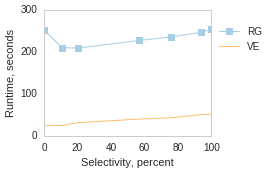
\includegraphics[width=2.8in]{figs/select_wikitalk_vertices_build12.png}
\caption{Select on the wikitalk dataset, return vertices.}
\vspace{-0.1in}
\label{fig:selectv}
\vspace{-0.1in}
\end{minipage}
\begin{minipage}{3.3in}
\centering
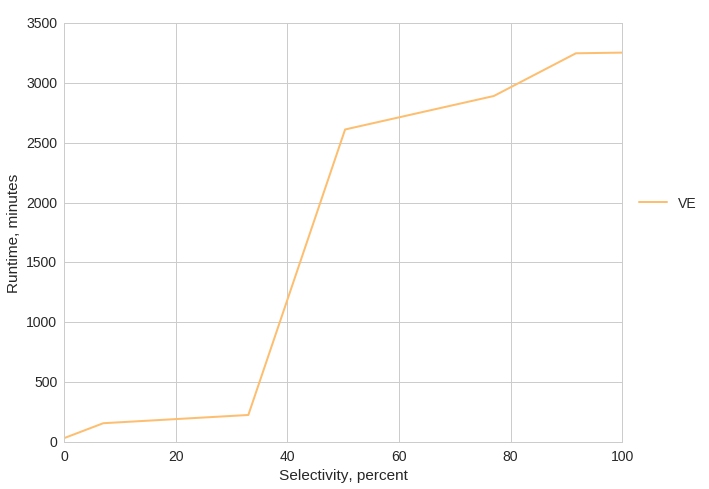
\includegraphics[width=2.8in]{figs/select_ngrams_edges_build12.png}
\vspace{-0.1in}
\caption{Select on the nGrams dataset, return edges.}
\vspace{-0.1in}
\label{fig:selecte}
\end{minipage}
\end{figure*}

{\bf Subgraph.}  \insql{subgraph} performance was evaluated by varying
selectivity over length of the vertex attribute.  When materializing
vertices, regardless of the evolution rate \ve provides better
performance than \sg and linear to selectivity.  Performance of \sg is
a function of the number of intervals and is insensitive to
the selectivity.  The behavior of \ve for edges
(Figure~\ref{fig:selecte}) is dominated by the foreign key constraint
enforcement: with small selectivity broadcast join affords performance
linear to the number of edges.  For large number of vertices broadcast
join is not feasible and a hash-join is used instead, which is
substantially slower.  Even then \ve provides an order of magnitude
better performance than \sg.

\eat{
\begin{figure}
\centering
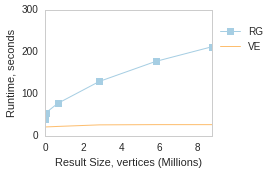
\includegraphics[width=2.8in]{figs/project_wikitalk_vertices_build12.png}
\caption{Project vertex attribute into its length on the wikitalk dataset.}
\label{fig:project}
\end{figure}
}
{\bf Project.}  We evaluate \insql{project} performance by varying the
data size through the slice operation.  Similar to \insql{slice},
\insql{project} exhibits flat runtime for \ve and linear increase in
runtime with the number of RGs for \sg.  However, performance for \ve
is worse than performance on \insql{slice} because \insql{project}
requires a coalescing operation as the last step, while \insql{slice}
does not.

\begin{figure*}[h]
\begin{minipage}{2in}
\centering
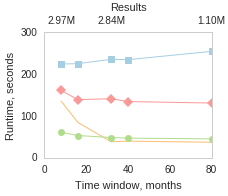
\includegraphics[height=1.7in]{figs/agg_allall_wikitalk_vertices_build11_trimmed.png}
\caption{Aggregate by time, all/all quantification on the wikitalk dataset.}
\label{fig:agg1}
\end{minipage}
\begin{minipage}{2in}
\centering
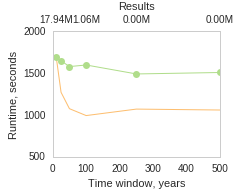
\includegraphics[height=1.7in]{figs/agg_allall_ngrams_edges_build11_trimmed.png}
\caption{Aggregate by time, all/all quantification on the nGrams dataset.}
\label{fig:agg2}
\end{minipage}
\begin{minipage}{2.6in}
\centering
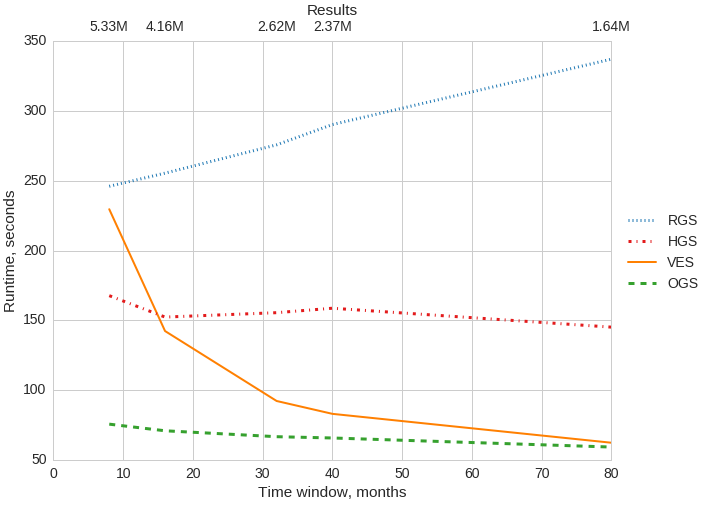
\includegraphics[height=1.7in]{figs/agg_allexists_wikitalk_edges_build11.png}
\caption{Aggregate by time, all/exists quantification on the wikitalk dataset.}
\label{fig:agg4}
\end{minipage}
\end{figure*}

\eat{
\begin{figure*}
\centering
\begin{minipage}{3.2in}
\centering
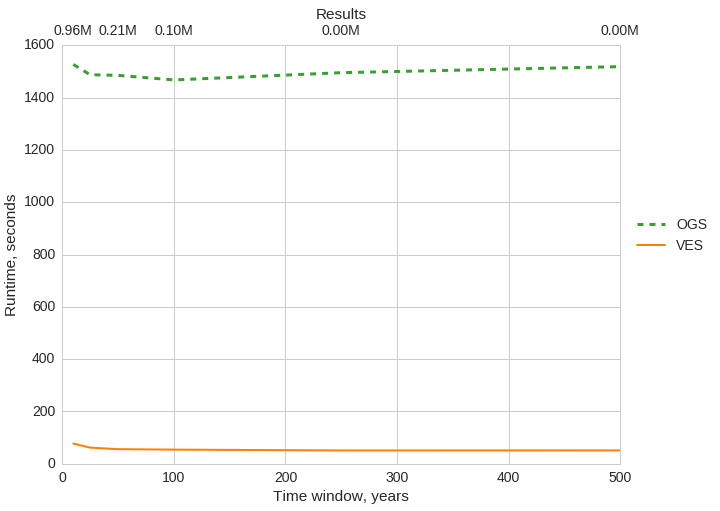
\includegraphics[width=3in]{figs/agg_allexists_ngrams_vertices_build11.png}
\vspace{-0.1in}
\caption{Aggregate by time, all/exists quantification on the nGrams dataset.}
\label{fig:agg3}
\vspace{-0.1in}
\end{minipage}
\begin{minipage}{3.2in}
\centering
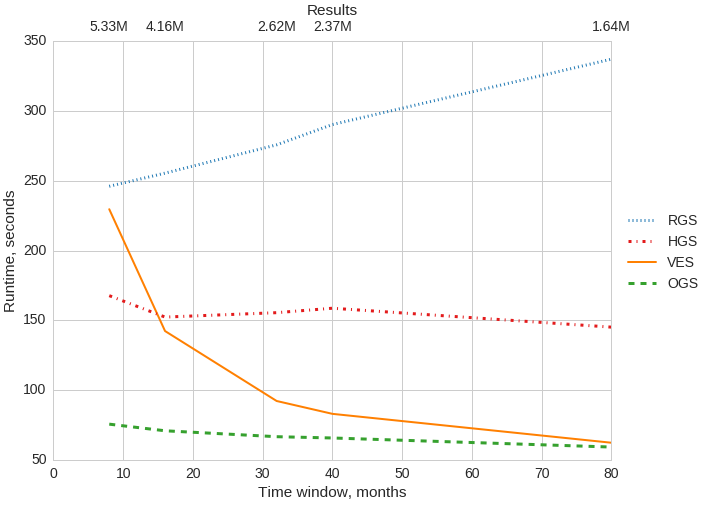
\includegraphics[width=3in]{figs/agg_allexists_wikitalk_edges_build11.png}
\vspace{-0.1in}
\caption{Aggregate by time, all/exists quantification on the wikitalk dataset.}
\label{fig:agg4}
\vspace{-0.1in}
\end{minipage}
\end{figure*}
}
{\bf Aggregate.}  We evaluate the performance of structure-only
aggregation on all 4 representations by varying the aggregation
window.  \insql{aggregate} performance, whether by time or change,
depends heavily on the quantification and on the data evolution rate.
\og is an aggregated data structure with good temporal locality and
thus in most cases provides good performance insensitive to the
aggregation window size, e.g. Figure~\ref{fig:agg1}.  However, in
datasets with a large number of RGs (such as nGrams which has over 400
periods), \og exhibits slow performance, an order of magnitude worse
than VE, except when materializing edges on small aggregation windows
(Figure~\ref{fig:agg2}).  \ve outperforms \og when the V and E
quantification levels match (Figure~\ref{fig:agg2}), but is worse than
\og when the foreign key constraint is manually enforced, which
happens with different levels of quantification for V and E
(Figure~\ref{fig:agg4}).  \ve also underperforms \og
when the evolution rate and the aggregation window are both small,
such as with the wikitalk dataset - Figure~\ref{fig:agg1}.  \sg and
\hg do not provide the best performance on any of our datasets.

\begin{figure*}[h]
\centering
\begin{minipage}{3.3in}
\centering
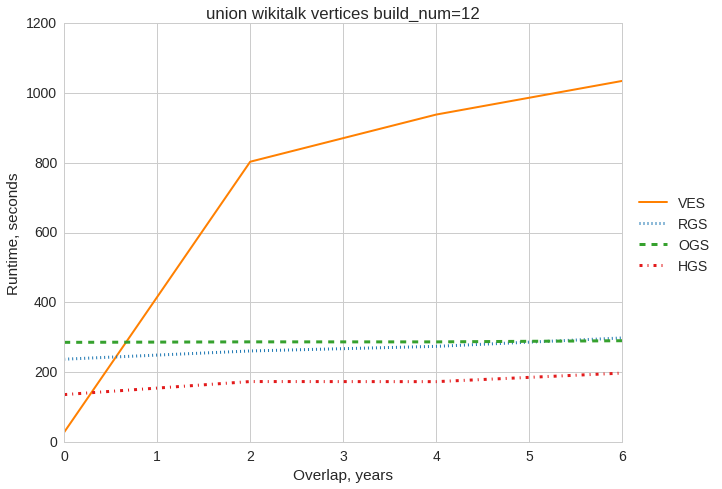
\includegraphics[width=2.8in]{figs/union_wikitalk_vertices_build12.png}
\caption{Union on the wikitalk dataset, return vertices.}
\label{fig:union1}
\end{minipage}
\begin{minipage}{3.3in}
\centering
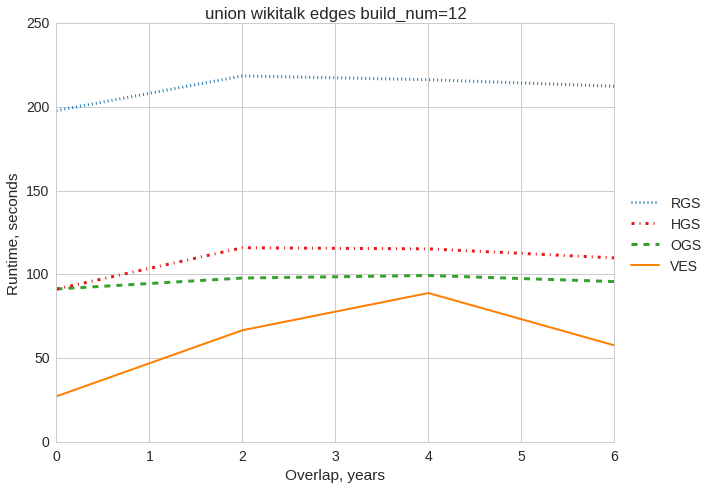
\includegraphics[width=2.8in]{figs/union_wikitalk_edges_build12.png}
\caption{Union on the wikitalk dataset, return edges.}
\label{fig:union2}
\end{minipage}
\end{figure*}

{\bf Union and Intersection.}  \insql{union} and \insql{intersection}
by structure was evaluated by loading two time slices of the same
dataset with varying overlap.  The performance of the four conditions
depends on the size of the overlap and the evolution rate.  \ve
produces the best performance when the overlap is small
(Figure~\ref{fig:union1}) and when the evolution rate is high
(Figure~\ref{fig:union2}), regardless of the size of the overlap.
\vera{MORE HERE}

\begin{figure*}[h]
\centering
\begin{minipage}{3.3in}
\centering
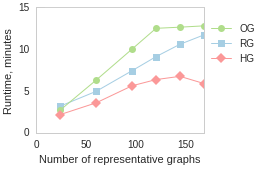
\includegraphics[width=2.8in]{figs/cc_wikitalk_build12.png}
\caption{Connected components on the wikitalk dataset.}
\label{fig:ccwiki}
\end{minipage}
\begin{minipage}{3.3in}
\centering
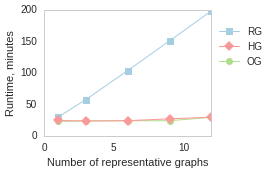
\includegraphics[width=2.8in]{figs/prank_twitter_build12.png}
\caption{Pagerank on the twitter dataset.}
\label{fig:pranktwitter}
\end{minipage}
\end{figure*}

{\bf Analytics.}  We implemented PageRank and Connected Components
analytics for the three graph-based representations using the Pregel
GraphX API.  PageRank was executed for 10 iterations or until
convergence, whichever came first.  Connected components was executed
until convergence with no limit on the number of iterations.
Performance of Pregel-based algorithms depends heavily on the
partition strategy, with best results achieved where cross-partition
communication is small.  For this reason, we evaluated only with the
E2D strategy.

The performance was evaluated on time slices of varying size.  For a
very small number of RGs (1-2), \sg provides good performance.
However, \sg performance slows down linearly with the number of RGs.
\hg provides the best performance on analytics under most conditions,
with a linear increase with a significantly slower rate of growth.
The tradeoff between \og and \hg depends on graph evolution
characteristics.  If the graph is a growth-only evolution (such as in
our twitter dataset), \og is not denser than \hg and computes
everything in a single batch mode, which leads to the fastest
performance, as can be seen in Figure~\ref{fig:pranktwitter}.  If the
edge evolution represents more ephemeral connections that can come and
go, then \hg is less dense and scales better
(Figure~\ref{fig:ccwiki}).

talk about how here for all 3 the graphs were RGs, not structure RGs. further gains can be head where structure evolution is slower than attrib. evolution

{\bf Cluster Size.}  We next examine how the system implementation
scales with the the size of the cluster.  We evaluate the performance
of two queries.

\begin{small}
\begin{verbatim}
Q1. wikitalk

   slice(2005-2015)
   aggregate(1 year, exists, exists)
   connected components
   materialize vertices
\end{verbatim}
\end{small}

This query, executed on the wikitalk dataset, computes connected
components over the past 10 years on the yearly scale.

\begin{small}
\begin{verbatim}
Q2. UKDELIS

   aggregate(3 months, exists, always)
   pagerank(20 iterations)
   project pagerank score
   aggregate(12 months, exists, exists, trend)
   get top 10
\end{verbatim}
\end{small}

This query, executed on DELIS dataset, computes stable links between
websites, i.e. links that persist for 3 months, and uses them to
compute pagerank for each.  The score is projected and its trend
computed in an aggregation over the whole dataset time period (1
year).  The top 10 websites with the highest increase in pagerank are
returned.

For each operation, the best performing representation was selected
based on our experimental results.  Slice, project, and aggregate were
performed with VE, analytics with \hg.  The results are in
Table~\ref{tab:clustersize}.

\begin{table}
\caption{Effect of cluster size.}
\small
\begin{tabular}{| l | c | r |}
\hline
\multicolumn{1}{|l|}{\bfseries Cluster Size} & \multicolumn{1}{c|}{\bfseries Q1} & \multicolumn{1}{r}{\bfseries Q2} \\ \hline
2 & ? & ? \\ \hline
4 & ? & ? \\ \hline
8 & ? & ? \\ \hline
12 & ? & ? \\ \hline
16 & ? & ? \\ \hline
\end{tabular}
\label{tab:clustersize}
\end{table}
